% copyright arturo salinas-aguayo 2025
\documentclass[12pt]{article}

\usepackage{graphicx}
\usepackage{subcaption}
\usepackage{amsmath}
\usepackage{siunitx}
\usepackage{array}
\usepackage{amsfonts}
\usepackage{fancyhdr}
\usepackage{geometry}
\usepackage{circuitikz}
\usepackage{caption}
\usepackage{bm}
\usepackage{float}

\geometry{letterpaper, margin=1in}
\graphicspath{ {../../images/} }

% Header and Footer
\pagestyle{fancy}
\fancyhf{}
\fancyhead[L]{ECE 2001 - Design Project 02: Audio Equalizer}
\fancyhead[R]{\thepage}
\setlength{\headheight}{15pt}

\author{Arturo Salinas-Aguayo}
\title{Design Project 02: Audio Equalizer}

% theorem set
\newtheorem{example}{Example}
% Example block environment
\newenvironment{examp}
{\vspace{0.5cm}
 \hrule
\vspace{0.5cm}
\begin{example}}
{\hrule
\vspace{0.5cm}
\end{example}}

\begin{document}
\newcommand{\closure}[2][3]{%
	{}\mkern#1mu\overline{\mkern-#1mu#2}}
\newcommand\ncoverline[1]{\mkern1mu\overline{\mkern-1mu#1\mkern-1mu}\mkern1mu}
% Title Page
\begin{titlepage}
	\centering
	\vspace*{3cm}
	\huge\textbf{Design Project 02: Audio Equalizer}\\

	\vspace{5cm}
	\Large\textbf{Arturo Salinas-Aguayo}\\
	\normalsize
	ECE 2001 Electrical Circuits\\
	Dr. David J. Giblin, Section 331.660.701.810-1253\\
	Mechanical Engineering Department
	\vfill
	
\includegraphics[scale=0.1]{uconnlogo}\\
	College of Engineering, University of Connecticut\\
	\scriptsize{Coded in \LaTeX}
	\vspace*{1cm}
\end{titlepage}
\tableofcontents
\newpage

\section{Abstract}
After being introduced to sinusoidal sources and reactive components in depth, the final project involves developing a more advanced music mixer that is capable of being tuned to attenuate or amplify certain frequencies.

There are many different applications when it comes to this vital tool, such as overboomy rooms at weddings, that leave speech muddy and unclear, to tuning a symphony hall's active speakers to bring out only the string instruments, without being too obvious that the instruments were indeed being amplified.

More recently, as cars have gotten better at dampening road noise and internal combustion engines are becoming smaller, companies such as GM and BMW are even tuning their sound systems to attempt to fool their customers that they are hearing the engine compared to a synthesized sound.

In practicality, this design project allows the opportunity to build on skills learned throughout the semester, starting with the build up on passive components, utilizing operational amplifiers, and then ending with the integration of reactive components such as inductors and capacitors.

\newpage
\section{Introduction}
Audio systems of days passed used to be synonymous with the graphic equalizer shown in Figure \ref{fig:equalizer}.

\begin{figure}[H]
	\centering
	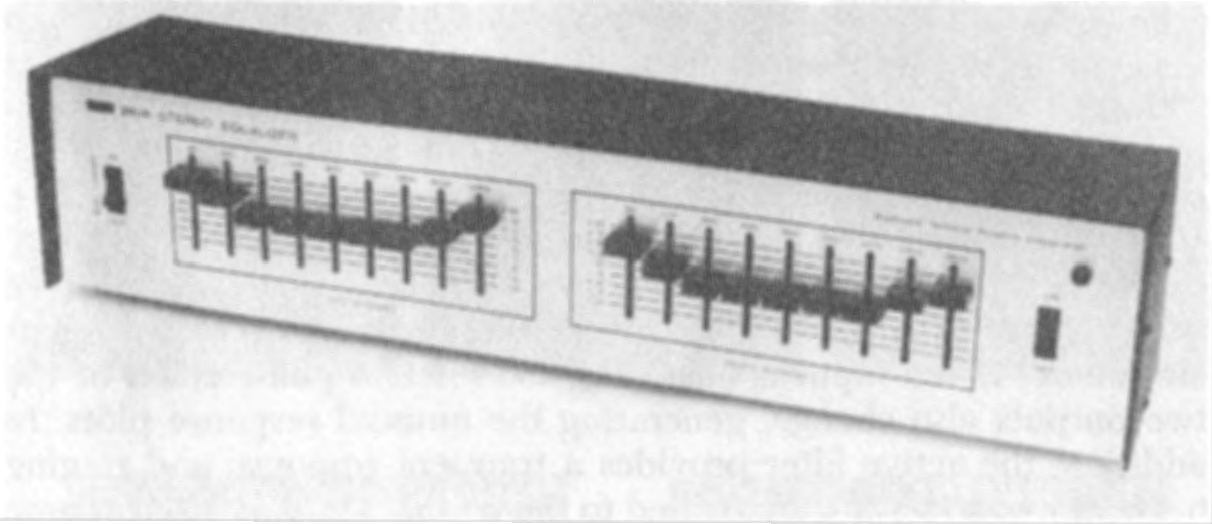
\includegraphics[width=\textwidth]{equalizer}
	\caption{Graphic Equalizer using eighteen active filters}
	\label{fig:equalizer}
\end{figure}
These consist of a bank of slide potentiometers that emphasize or de-emphasize portions of the audio spectrum such that all purpose speakers can be \textit{tuned} to their surrounding environment according to the listener (customer's) preferences. Often, these are made of low-Q, active bandpass filters such as the ones employed here. A sample circuit is shown in Figure \ref{fig:equalizercircuit}.
\begin{figure}[H]
	\centering
	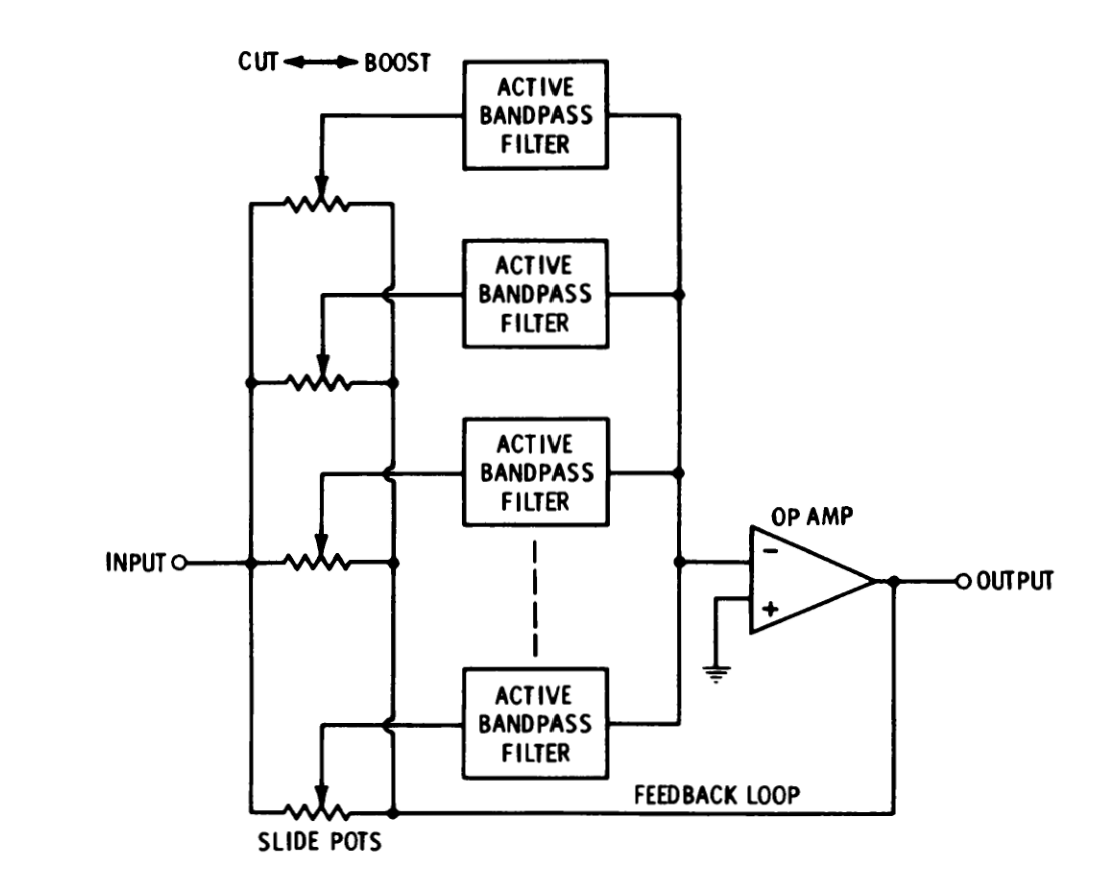
\includegraphics[width=8cm]{equalizercircuit}
	\caption{Graphic Equalizer with Multiple Active Filters in a Loop}
	\label{fig:equalizercircuit}
\end{figure}
These equalizers provide the  ability to ``boost" or ``cut" operation where each slide control provides a flat response in the middle of its range and provide progressively more emphasis or de-emphasis as the limits of the slider are approached.

This design employs some constraints such that the ranges and frequency response is set. A Quality Factor or Q value is also set which determines the slope of the filter at its peaks, or how wide the response is.
\begin{figure}
	\centering
	\begin{tabular}{|c|c|}
		\hline
		Parameter & Value(s) \\
		\hline
		Supply Voltage & $\pm 5V$\\
		\hline
		Bass Band & Center Frequency = $200 Hz \pm 10\%$

	\end{tabular}
\end{figure}


\section{Theory}
\subsection{Frequency Range and Q}
With active filters, the useful frequency range is far wider than for any other
filtering technique. The practical lower limit for a filter is somewhere between $0.01$ and $0.1Hz$, where the limiting component is the capacitor size.

The upper limit on frequency is set by the quality of the operational amplifier used. In this case, the $\mu A741$ is used again, which is notoriously out of date. This puts the upper limit in the $100KHz$ to $1MHz$ range. Above these frequencies, the conventional inductor-capacitor filters drop enough in size and cost that they are more practical than operational amplifiers.

When considering Bandpass filters, the narrowness or range of response can also be tuned. This bandwidth of a single filter structure is called its Q and is the ratio of its bandwidth to its center frequency. For example,
\begin{align*}
	f_c &= 200Hz \\
	f_b &= 2Hz \\
	Q &= \frac{200}{2} = 100
\end{align*}
\subsubsection{Bandwidth}
The bandwidth of a filter is defined as the difference betweeen the upper and lower points of where the filter response finally falls to 3dB below its peak value on the way out of the passband.

\subsubsection{Normalization}
A normalized filter is one such that its component values are adjusted to a convenient frequency and impedance level.

\subsubsection{Cutoff Frequency}
The cutoff frequency is the final point at which the filter response drops by $3 dB$ or approximately $0.707$ of its peak value on the way out of the passband.

\subsection{Multiple-Feedback (MFB) Bandpass Filter}
This project employs the exclusive use of the MFB Bandpass filter in order to tune and achieve the design characteristics. The practical limitations of a single stage MFB are such that the Q of the circuit is limited to quite low Q values.

\begin{figure}[H]
	\centering
	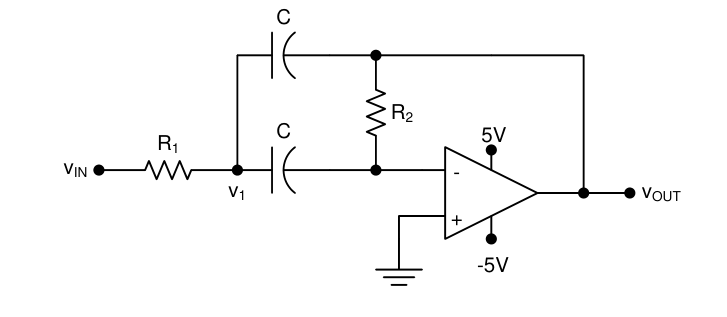
\includegraphics[width=0.75\textwidth]{07_multfeed}
	\caption{Multiple-Feedback Bandpass Filter.}
	\label{fig:multfeed}
\end{figure}

The MFB bandpass filter is another second-order topology but arranges two
resistors and two capacitors in a specific feedback loop. The transfer function can be derived using the node voltage method as such: ($s = j\omega$)
\begin{equation*}
	H(s) \;=\;
	\frac{-sR_2C}
	{s^2R_1R_2C^2 + 2sR_1C + 1}
\end{equation*}

which may be rewritten to match a standard second-order bandpass form:
\begin{align*}
	f_0 & = \frac{1}{2\pi\,C\sqrt{R_1R_2}}     \\
	A_r & = -\frac{R_2}{2R_1}                 \\
	Q   & = \frac{1}{2}\sqrt{\frac{R_2}{R_1}}
\end{align*}
By choosing $R_1$, $R_2$, and $C$, one can specify the center frequency $f_0$ and
quality factor $Q$. Because the peak amplitude occurs at $f_0$, we say the
bandwidth $\mathrm{BW}$ is bounded by the $-3\,\mathrm{dB}$ frequencies, and for
a standard bandpass $Q = \tfrac{f_0}{\mathrm{BW}}$.
\subsection*{Tuning the MFB Bandpass Filter}
Tuning each of the desired frequencies is simply a matter of following Figure \ref{fig:tuning}.

\begin{figure}[H]
	\centering
	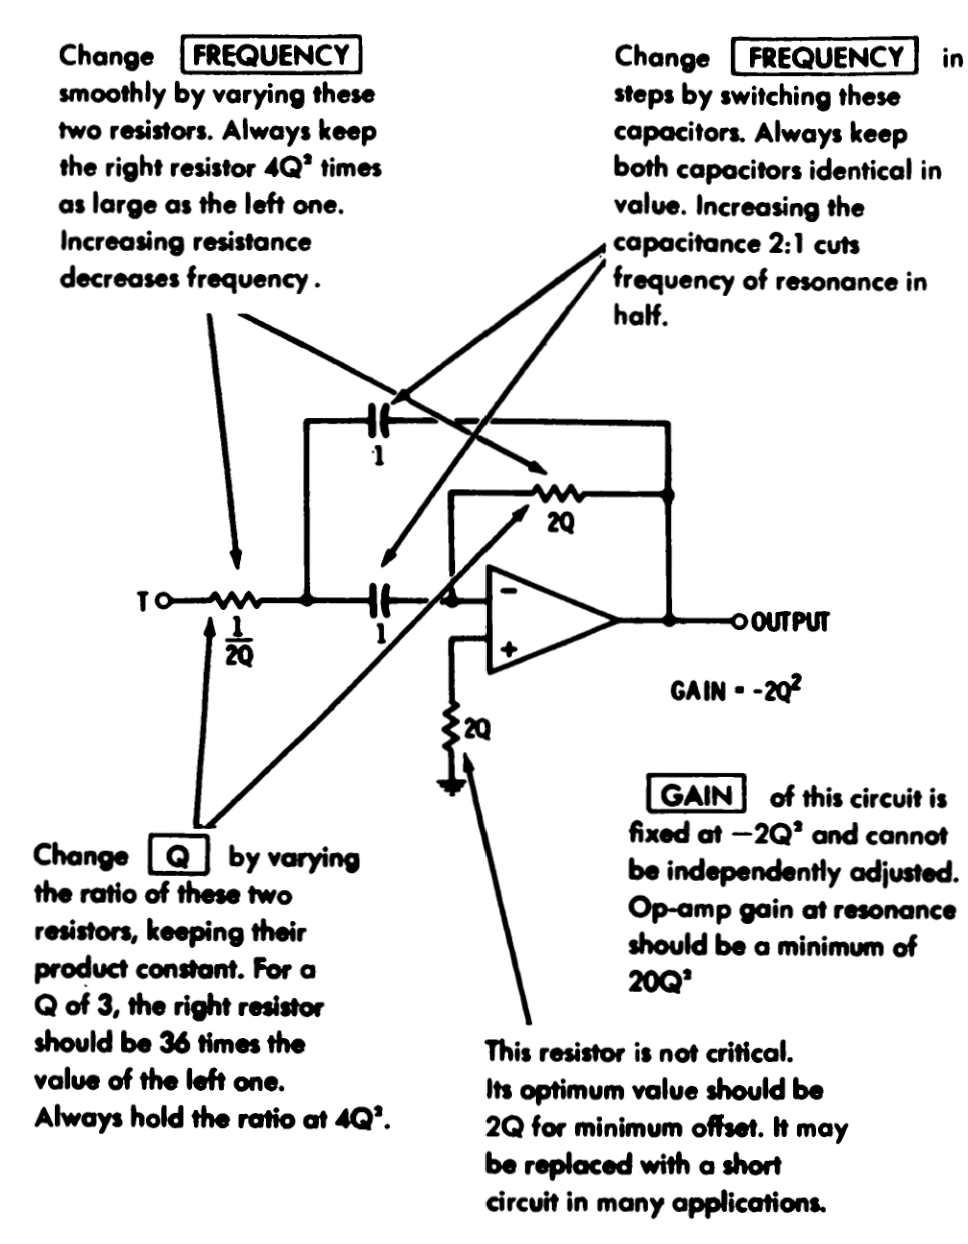
\includegraphics[width=0.5\textwidth]{tuning}
	\caption{Tuning a Multiple-Feedback Bandpass Filter.}
	\label{fig:tuning}
\end{figure}
To begin the tuning and design of the circuit, first the Q factor is considered. Recall,
\[
	Q = \frac{1}{2}\sqrt{\frac{R_2}{R_1}}
\]
All three of the frequency ranges are designed to the same Q of $0.7 \pm 10\%$ or
	\[
		1.96 = \frac{R_2}{R_1}
	\]

Essentially, this means that as long as the ratio remains constant, the Q will be achieved.
Designing for specifying center frequencies is a matter of choosing a capacitor for the target and then finding a standard resistor ratio that will satisfy it.

To achieve this, the same resistors were used for all three MFB stagess:
\begin{align*}
	R_2 &= 10k\Omega\\
	R_1 &= 5.1k\Omega
\end{align*}

\subsection{Bass Band}
\noindent \textbf{Specifications:}
\begin{itemize}
	\item Center Frequency - 200Hz
	\item Quality Factor - 0.7
	\item Range of Adjustable Gain 0.4 - 8
\end{itemize}
Utilizing:
\begin{align*}
	f_0 & = \frac{1}{2\pi\,C\sqrt{R_1R_2}}     \\
	200 & = \frac{1}{2\pi\,C\sqrt{5100\cdot10000}}\\
	C & \approx 110nF\\
\end{align*}
\subsection{Midrange Band}
\noindent \textbf{Specifications:}
\begin{itemize}
	\item Center Frequency - 1.0kHz
	\item Quality Factor - 0.7
	\item Range of Adjustable Gain - 0.2 - 4
\end{itemize}
Utilizing:
\begin{align*}
	f_0 & = \frac{1}{2\pi\,C\sqrt{R_1R_2}}     \\
	1000 & = \frac{1}{2\pi\,C\sqrt{5100\cdot10000}}\\
	C & \approx 22nF\\
\end{align*}
\subsection{Treble Band}
\noindent \textbf{Specifications:}
\begin{itemize}
	\item Center Frequency - 5.0kHz
	\item Quality Factor - 0.7
	\item Range of Adjustable Gain 0.1 - 2
\end{itemize}
Utilizing:
\begin{align*}
	f_0 & = \frac{1}{2\pi\,C\sqrt{R_1R_2}}     \\
	5000 & = \frac{1}{2\pi\,C\sqrt{5100\cdot10000}}\\
	C & \approx 4.7nF\\
\end{align*}
The results of this simulated in SPICE can be seen  in Figure \ref{fig:mfbstage}.
\begin{figure}[H]
	\centering
	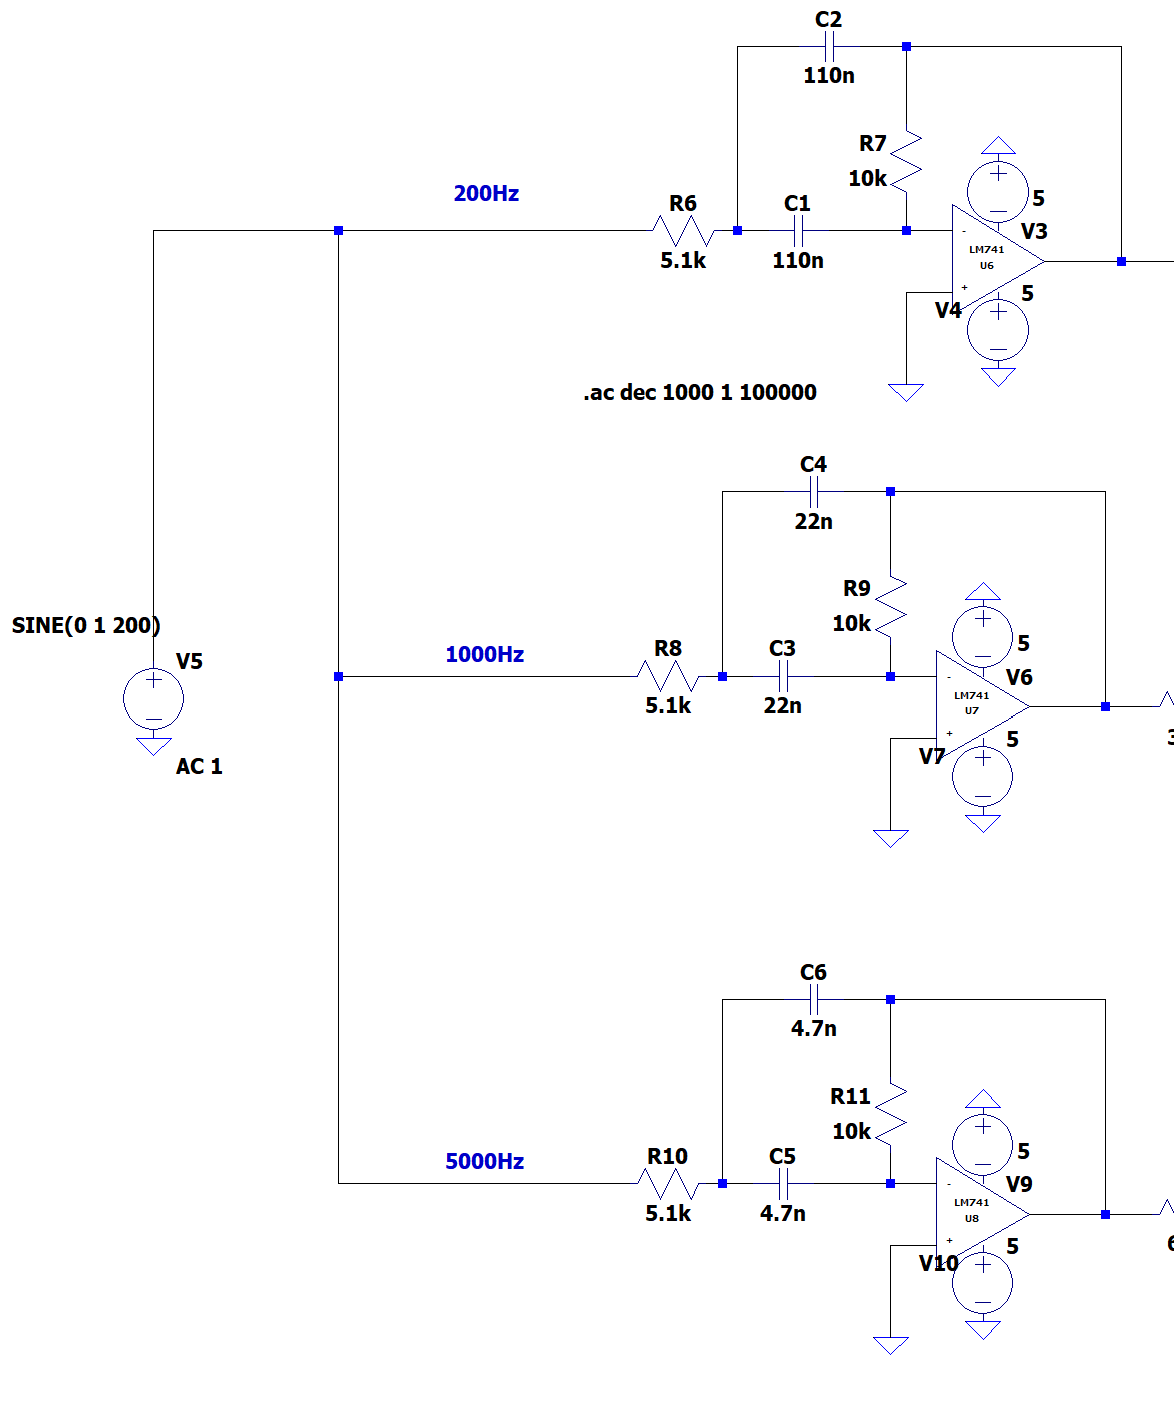
\includegraphics[width=0.8\textwidth]{mfbstage}
	\caption{Frequency Selection Stage}
	\label{fig:mfbstage}
\end{figure}
\subsection{Amplification}
This leaves the matter of amplifying and allowing for the adjustment of the normalized gain of the circuit.
\section{Experimental Procedures}

\section{Results and Discussion}

\section{Conclusion}
\end{document}
% vim: set ft=tex tw=80 ts=2 sts=2 sw=2 noet spell:
